\section{FriendLocator} % Bookmark information

\begin{frame}[red]
\frametitle{\textsc{FriendLocator}}
\begin{center}
\Large\textsc{FriendLocator} - A Location Privacy Aware Friend Locator
\end{center}
\end{frame}

\subsection{Core idea}
\begin{frame}[red]
\frametitle{Core idea of \textsc{FriendLocator}}
\only<1>{ 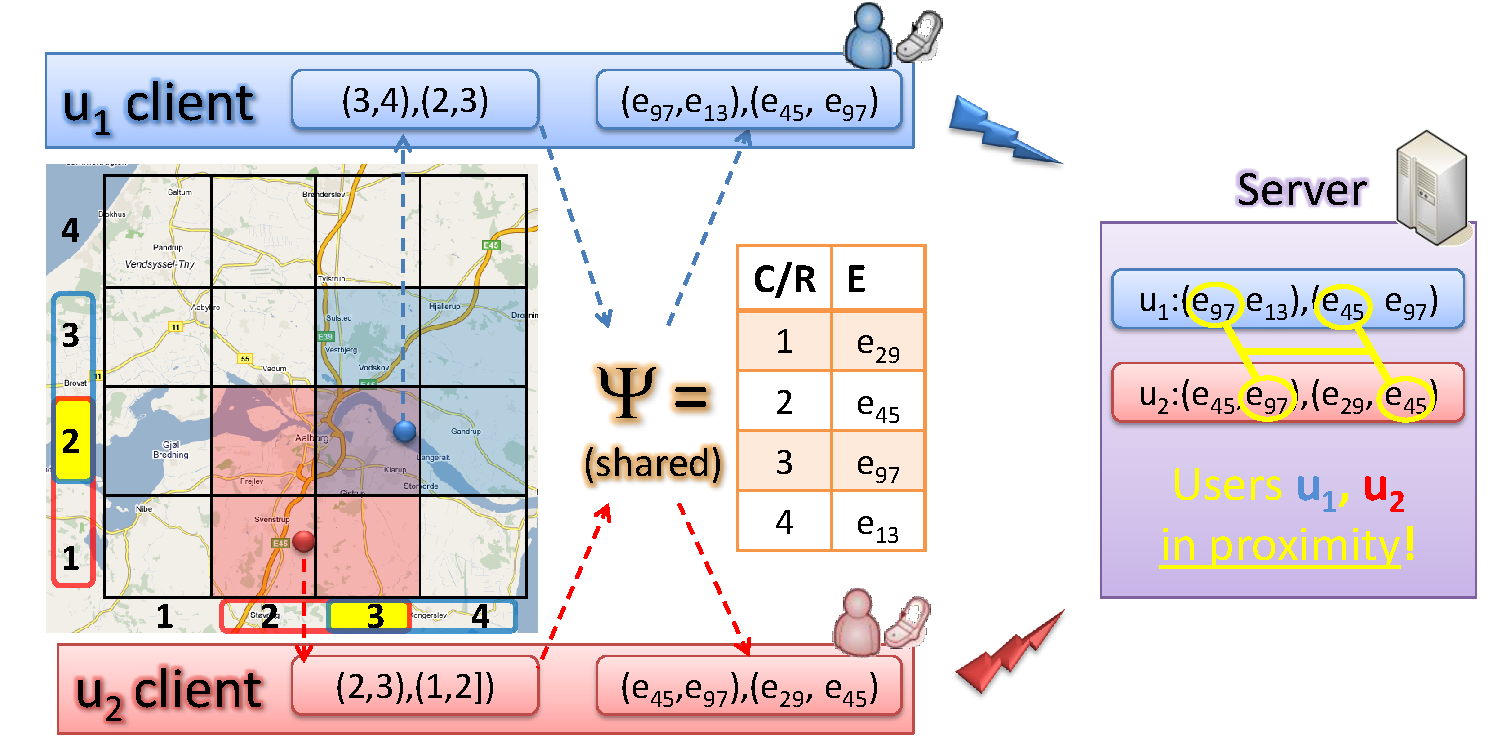
\includegraphics[scale=0.45]{images/ffBehaviour.pdf}}
\only<2>{ \includegraphics[page=7,scale=0.55]{images/imagesLRS.pdf}}
\only<3>{ \includegraphics[page=8,scale=0.55]{images/imagesLRS.pdf}}
\only<4>{ \includegraphics[page=9,scale=0.55]{images/imagesLRS.pdf}}
\only<5>{ \includegraphics[page=10,scale=0.55]{images/imagesLRS.pdf}}
\end{frame}

\begin{frame}[red]
\frametitle{Limitation and extensions of the idea}
Limitations of the core idea:
\begin{enumerate}
 \item Intercepted $\Psi$ opens location privacy leakage possibility
 \item A proximity detection distance is fixed ($2d\sqrt{2}$)  
\end{enumerate}
	\begin{tabular}{p{5cm} p{4cm}} 
	   \includegraphics[scale=0.2]{images/usrSrvAdversary.pdf} &
	   \includegraphics[scale=0.2]{images/usrPosDemoA.pdf} 
	\end{tabular}
	
Extensions, supported by \textsc{FriendLocator}:
\begin{enumerate}
   \item Grouping of friends
   \item Incremental Proximity Detection Approach
\end{enumerate}
\end{frame}

\subsection{Grouping of friends}

\begin{frame}[red]
\frametitle{Grouping of friends}
 Solution:
	\begin{itemize}
	\item Users are grouped into friend-groups			  
	\item A distinct $\Psi$ is assigned for every friend-group
	\end{itemize}
\begin{center}
  \includegraphics[page=11,scale=0.3]{images/imagesLRS.pdf}
\end{center}	
\vspace{-1cm}
Consequences:
	\begin{itemize}
	\item When user becomes malicious, users from common groups are endangered
	\end{itemize}
\end{frame}

\subsection{Incremental Proximity Detection Approach}
\begin{frame}[red]
\frametitle{Incremental Proximity Detection Approach}
\only<1>{
The solution:
	\begin{itemize}
	\item A list of grids with decreasing cell size is assigned for every friend-group
	\end{itemize}
\begin{center}
  \includegraphics[scale=0.2]{images/proxDet3.pdf} 
\end{center}	
Consequences:
	\begin{itemize}
	\item Any pair of friends in friend-group will be able to choose a preferred proximity distance
	\end{itemize}
}
\only<2>{\includegraphics[page=13,scale=0.55]{images/imagesLRS.pdf}}
\only<3>{\includegraphics[page=14,scale=0.55]{images/imagesLRS.pdf}}
\only<4>{\includegraphics[page=15,scale=0.55]{images/imagesLRS.pdf}}
\only<5>{\includegraphics[page=16,scale=0.55]{images/imagesLRS.pdf}}
\only<6>{\includegraphics[page=17,scale=0.55]{images/imagesLRS.pdf}}
\only<7>{\includegraphics[page=18,scale=0.55]{images/imagesLRS.pdf}}
\only<8>{\includegraphics[page=19,scale=0.55]{images/imagesLRS.pdf}}
\end{frame}
